% !TeX program = lualatex
\documentclass[final]{beamer}
\usepackage[T1]{fontenc}
\usepackage{lmodern}
\usepackage[orientation=portrait, size=a1, scale=1.44]{beamerposter}
\usetheme{gemini}
\usecolortheme{exeter}
\usepackage{graphicx}
\usepackage{epstopdf}
% \usepackage{booktabs}

% Lengths
% If you have N columns, choose \sepwidth and \colwidth such that (N+1)*\sepwidth + N*\colwidth = \paperwidth
\newlength{\sepwidth}
\newlength{\colwidth}
\setlength{\sepwidth}{0.02\paperwidth}
\setlength{\colwidth}{0.47\paperwidth}
\newcommand{\separatorcolumn}{\begin{column}{\sepwidth}\end{column}}

	\title{%
  \texorpdfstring{%
		\makebox[\linewidth]{%
		\makebox[0pt][l]{%
		\raisebox{\dimexpr-\height+0.8\baselineskip-3.5cm}[0pt][0pt]
			{\hspace*{11.88mm}
\includegraphics[height=0.8\baselineskip]{images/exeter-logo.eps}}% Right logo
	}%    
	  \hfill%
      \makebox[0pt]{Can statistics help us to understand deep learning?}%
			\hfill
			\makebox[0pt][r]{%
			\raisebox{\dimexpr-\height+\baselineskip}[0pt][0pt]%
	}%
		}%  
		}%
	{Can statistics help us to understand deep learning?}
	}
\author{Hannes Smit}

\begin{document}
\begin{frame}[t]
	\vspace*{-1cm}
	\begin{columns}[t]
		\separatorcolumn
		\begin{column}{\colwidth}
			\begin{block}{Introduction}
				Since the turn of the millennium, machine learning, and particularly \textbf{deep learning} have been able to solve many problems that were once thought impossible for a computer.
				The complex nature of these algorithms means that they are opaque to human understanding.
				As these algorithms become more sophisticated and are applied to more real world tasks such as driving cars or making parole decisions in the U.S., it is becoming more important to be able to deconstruct an algorithm in a way that humans can examine it.
			\end{block}
			\begin{block}{Artificial Neural Networks}
				One type of machine learning algorithm is the \textbf{Artificial Neural Network} (ANN), which takes inspiration from biological brains.
				Each `neuron' in the algorithm performs a simple weighted sum which is passed to a nonlinear activation function.
				The output of the neurons on each layer is fed into the next layer of neurons until the information reaches the output neuron.
				The weights are optimised to fit the training data provided and can then be used to make predictions on unseen datasets.
				\begin{figure}
					\centering
					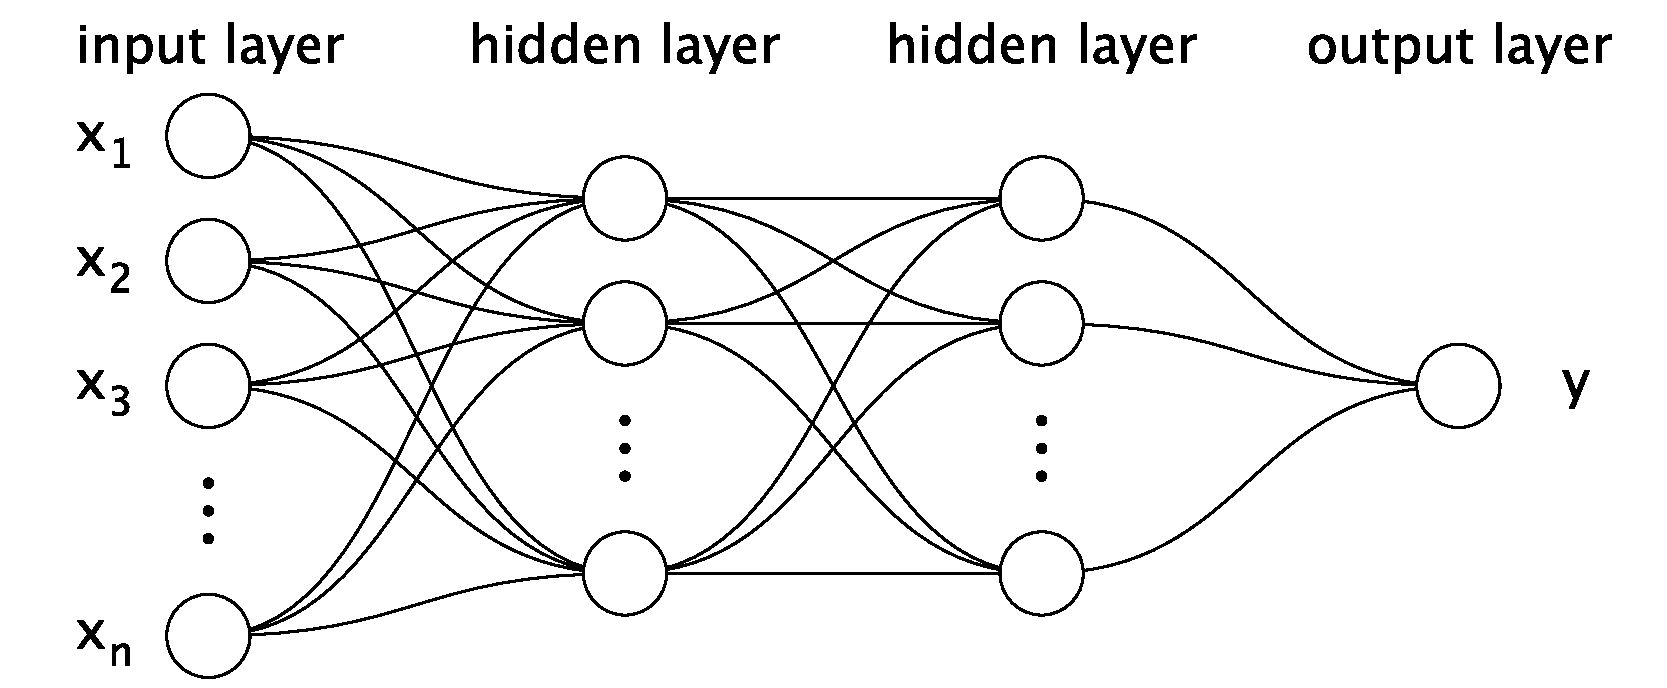
\includegraphics[width=0.75\textwidth]{images/nn-structure.pdf}
					\vspace*{-1cm}
					\caption{An example of a neural network's structure with two hidden layers.}
					\vspace*{-0.5cm}
				\end{figure}
				To use as a simple example, an ANN with 8 hidden layers, each with 10 neurons with a tanh activation, was trained on data following the pattern\ y\;=\;x\;+\;5\,sin(x)\,.
				\begin{figure}
					\centering
					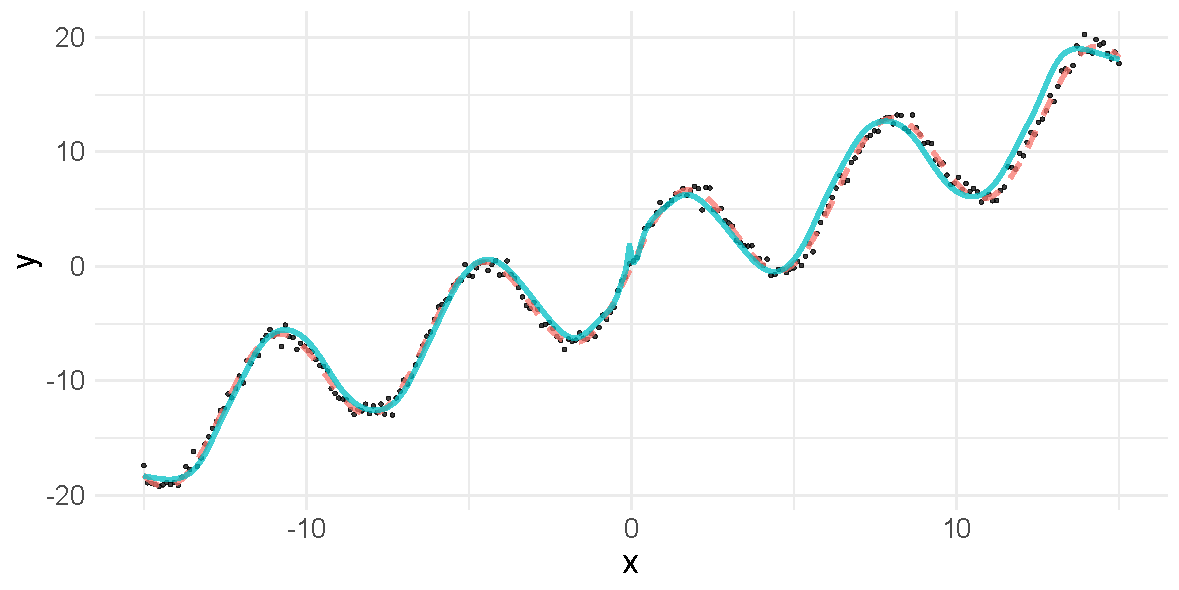
\includegraphics[width=\textwidth]{images/ann-trained.pdf}
					\vspace*{-2cm}
					\caption{The true function (dashed red), the training data (black), and the fit of the ANN (blue).}
					\vspace*{-0.5cm}
				\end{figure}
				One of the findings at this stage was that when training ANNs, the order of the datapoints can significantly affect the fit of the model due to the type of batch stochastic gradient descent used.
				Datapoints that are used later in the training process seem to have less impact on the model's predictions.
				\begin{figure}
					\centering
					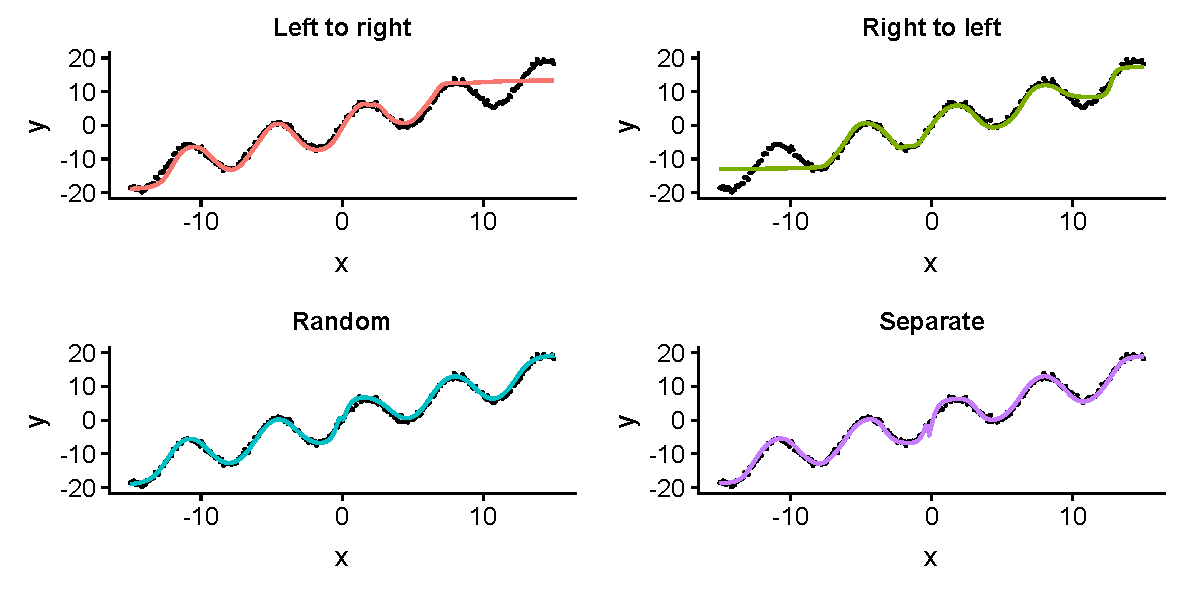
\includegraphics[width=\textwidth]{images/compare-nn-order.pdf}
					\vspace*{-2cm}
					\caption{Comparing the fit of the ANN with different ordering methods.}
					\vspace*{-0.5cm}
				\end{figure}
				To solve this, the order of the datapoints can be randomised or separated systematically (seen in blue and purple above respectively).
			\end{block}
		\end{column}
		\separatorcolumn
		\begin{column}{\colwidth}
			\begin{block}{Gaussian Processes}
				We can use \textbf{Gaussian Processes} (GPs) to try and model the output of the ANN.
				GPs are an extension of the multivariate normal distribution to an infinite dimensional process with a mean function and covariance function instead of a mean vector and covariance matrix.
				GPs are very flexible, so applying a GP to the output of the ANN is likely to result in a close fit.
				\begin{figure}
					\centering
					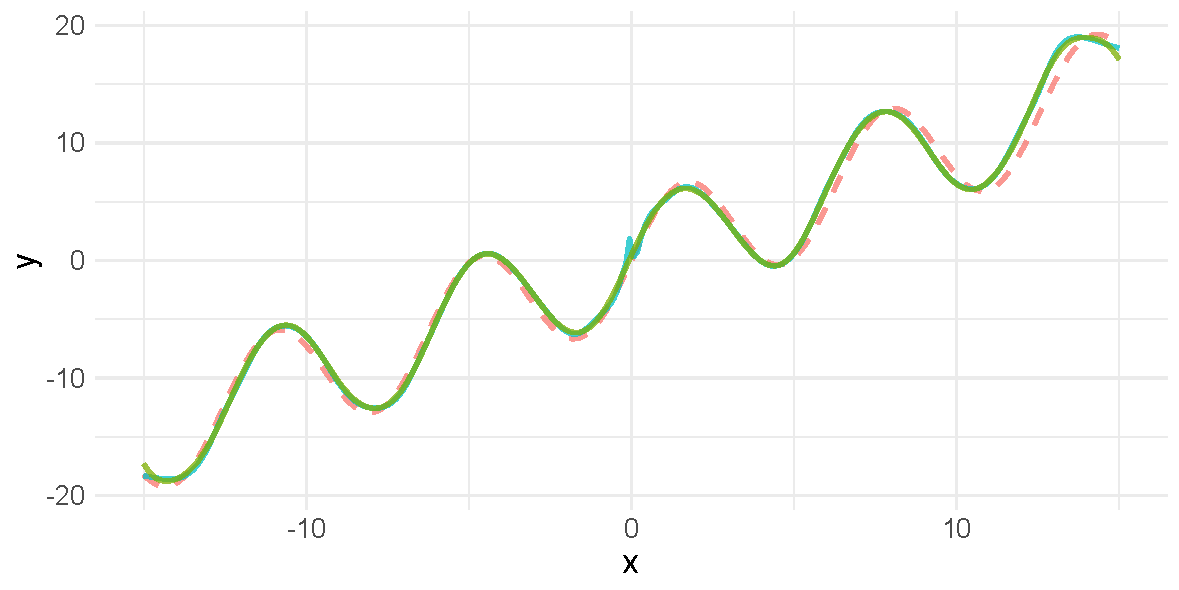
\includegraphics[width=\textwidth]{images/gp-trained.pdf}
					\vspace*{-1cm}
					\caption{The true function (dashed red), the fit of the ANN (blue) and the fit of the GP on the output of the ANN (green).}
					\vspace*{-0.5cm}
				\end{figure}
				GPs have some well understood statistical properties that allow us to learn more about the ANN.
			\end{block}
			\begin{block}{Stepwise Regression and LASSO}
				It is possible to use \textbf{stepwise regression} on the output of the ANN to try and identify the exact mathematical components that it is approximating.
				By fitting a linear model with the predictors x, x², sin(x), sin(2x), sin(x/2), cos(x), cos(2x) and cos(x/2), stepwise regression was able to reduce the model to a smaller one. 
				\begin{table}[ht]
					\centering
					\begin{tabular}{rrrrr}
						\hline
						            & Estimate & Std. Error & t value & p value \\
						\hline
						(Intercept) & -0.0048  & 0.0428     & -0.11   & 0.9114  \\
						x           & 1.0311   & 0.0033     & 310.07  & 0.0000  \\
						x²          & 0.0009   & 0.0004     & 2.24    & 0.0262  \\
						sin(x)      & 4.8708   & 0.0406     & 119.87  & 0.0000  \\
						sin(x/2)    & 0.1248   & 0.0418     & 2.98    & 0.0031  \\
						\hline
					\end{tabular}
				\end{table}
				While the relevant estimators x and sin(x) were identified and their coefficients fairly accurately estimated, a few other variables were also identified as significant.
				This method is only likely to work with a perfect or near perfect fit with no noise, which is unrealistic for real applications.
				
				Alternatively, we can use the \textbf{Least Absolute Shrinkage and Selection Operator} (LASSO) method to select the significant variables from the full model.
				\begin{table}[ht]
					\centering
					\begin{tabular}{rr}
						\hline
						variable    & coefficient \\
						\hline
						(Intercept) & 0.07        \\
						x           & 1.02        \\
						sin(x)      & 4.74        \\
						\hline
					\end{tabular}
				\end{table}
				The LASSO method successfully identified the significant variables and estimated their coefficients fairly accurately.
				However, both of these methods require some understanding of the ML algorithm to be able to choose relevant variables. 
			\end{block}
			\begin{block}{Future Research}
				This experiment has shown that it is possible to use methods to help understand machine learning, however much more research is required to find out how effective these methods can be. 
				\begin{itemize}
					\item Additional research could be done into using a stepwise regression or LASSO approach to capture the larger scale trend and then using that as a mean function for a GP to model the residuals.
					\item The next stage of research would be to test these methods on a more complex dataset and ML algorithm.
					      Even simple real life applications can have many dimensions and a non-repetitive structure.
				\end{itemize}
			\end{block}
		\end{column}
		\separatorcolumn
	\end{columns}
\end{frame}
\end{document}
